\documentclass[10.5pt,letterpaper]{article}
\usepackage[margin=0.7in]{geometry}
\usepackage{fontspec}
\setmainfont{Arial}
\usepackage{graphicx}
\usepackage{tikz}
\usetikzlibrary{calc,positioning,shapes.geometric}
\usepackage{xcolor}
\usepackage{tabularx}
\usepackage{array}
\usepackage{booktabs}
\usepackage{enumitem}
\usepackage{multicol}
\usepackage{titlesec}
\usepackage{fancyhdr}
\usepackage{hyperref}
\usepackage{tcolorbox}
\tcbuselibrary{skins,breakable}
\usepackage{microtype}
\usepackage{amssymb}

\definecolor{TDFPurple}{HTML}{8B5CF6}
\definecolor{TDFViolet}{HTML}{6D28D9}
\definecolor{TDFPink}{HTML}{F43F5E}
\definecolor{TDFInk}{HTML}{11111B}
\definecolor{TDFSlate}{HTML}{4B5563}
\definecolor{TDFMist}{HTML}{F6F3FF}
\definecolor{TDFLine}{HTML}{E9E2FF}
\definecolor{TDFGreen}{HTML}{0E9F6E}
\definecolor{TDFGold}{HTML}{D97706}

\hypersetup{colorlinks=true,linkcolor=TDFViolet,urlcolor=TDFViolet,pdftitle={Guía TDF: Eventos y Tickets},pdfauthor={TDF Records}}
\setlength{\parindent}{0pt}
\setlength{\parskip}{5pt}
\renewcommand{\arraystretch}{1.32}
\newcolumntype{Y}{>{\raggedright\arraybackslash}X}
\newcommand{\pill}[1]{\tikz[baseline=(X.base)]\node[fill=TDFMist,text=TDFViolet,rounded corners=8pt,inner xsep=7pt,inner ysep=3pt,font=\footnotesize\bfseries](X){#1};}
\newcommand{\step}[1]{\tikz[baseline=(X.base)]\node[fill=TDFPurple,text=white,circle,minimum size=18pt,inner sep=0pt,font=\small\bfseries](X){#1};}
\newcommand{\checkmarktdf}{\textcolor{TDFGreen}{\large\ensuremath{\checkmark}}}
\newcommand{\warn}{\textcolor{TDFGold}{\large\ensuremath{\blacktriangleright}}}

\titleformat{\section}{\Large\bfseries\color{TDFInk}}{}{0pt}{}
\titlespacing*{\section}{0pt}{16pt}{7pt}
\titleformat{\subsection}{\large\bfseries\color{TDFViolet}}{}{0pt}{}
\titlespacing*{\subsection}{0pt}{11pt}{4pt}
\pagestyle{fancy}
\fancyhf{}
\lfoot{\textcolor{TDFSlate}{TDF Records \;|\; Guía de Eventos y Tickets}}
\rfoot{\textcolor{TDFSlate}{\thepage}}
\renewcommand{\headrulewidth}{0pt}

\begin{document}
\begin{titlepage}
\thispagestyle{empty}
\begin{tikzpicture}[remember picture,overlay]
  \fill[TDFInk] (current page.south west) rectangle (current page.north east);
  \fill[TDFViolet] ($(current page.north east)+(-1.9in,-0.1in)$) circle (2.25in);
  \fill[TDFPink] ($(current page.south east)+(-0.15in,1.0in)$) circle (1.45in);
  \fill[TDFPurple,opacity=.35] ($(current page.south west)+(0.6in,0.25in)$) circle (1.5in);
  \draw[white,opacity=.12,line width=0.5pt] ($(current page.south west)+(0.55in,1.35in)$) -- ($(current page.north east)+(-0.55in,-1.35in)$);
\end{tikzpicture}
\vspace*{0.6in}

\includegraphics[width=2.05in]{tdf-hq-ui/public/tdf-logo-wordmark.png}\par
\vfill
{\color{white}\fontsize{30}{35}\selectfont\bfseries
Convierte una idea\\
en un evento que sucede.\par}
\vspace{0.24in}
{\color{white}\large Guía práctica para crear tu evento, configurar tickets y preparar la venta.\par}
\vspace{0.35in}
\pill{EVENTOS SOCIALES} \hspace{5pt}\pill{TICKETS} \hspace{5pt}\pill{JULIO 2026}
\vfill
{\color{white}\large\bfseries TDF Records}\par
{\color{white!70}\small Hecho para organizadores que cuidan cada detalle.}
\end{titlepage}

\begin{tcolorbox}[enhanced,arc=10pt,boxrule=0pt,colback=TDFMist,left=14pt,right=14pt,top=11pt,bottom=11pt]
\textcolor{TDFViolet}{\bfseries EN DOS MINUTOS}\quad Crea el evento, publica una ficha clara, agrega tipos de ticket y revisa cada venta desde el mismo lugar.
\end{tcolorbox}

\section*{Antes de empezar}
\begin{tabularx}{\textwidth}{@{}p{0.36in}Y@{\hspace{10pt}}p{0.36in}Y@{\hspace{10pt}}p{0.36in}Y@{}}
\checkmarktdf & Inicia sesión en TDF. & \checkmarktdf & Ten lista la fecha, venue y aforo. & \checkmarktdf & Prepara un afiche o foto nítida. \\
\end{tabularx}

\begin{tcolorbox}[enhanced,breakable,colback=white,colframe=TDFLine,boxrule=.8pt,arc=10pt,left=14pt,right=14pt,top=10pt,bottom=11pt,title=Ruta rápida,coltitle=TDFViolet,fonttitle=\bfseries]
Desde el menú lateral entra a \textbf{Social → Eventos sociales}. También puedes abrir directamente \href{https://tdf-app.pages.dev/social/eventos}{tdf-app.pages.dev/social/eventos}. El creador del evento queda como organizador y ve los controles de tickets y órdenes.
\end{tcolorbox}

\section*{El flujo, de un vistazo}
\begin{center}
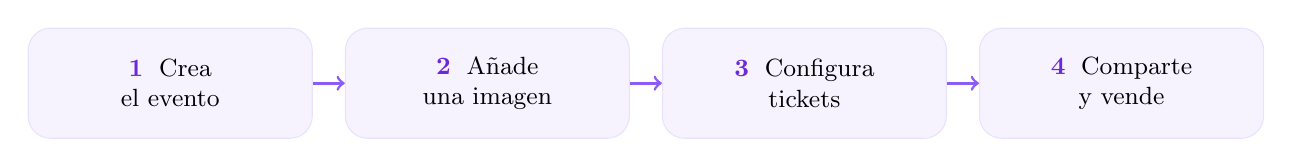
\begin{tikzpicture}[node distance=0.25in and .16in, every node/.style={font=\small}]
\node[draw=TDFLine,fill=TDFMist,rounded corners=8pt,minimum width=1.42in,minimum height=.55in,align=center] (a) {\textcolor{TDFViolet}{\bfseries 1}\; Crea\\el evento};
\node[draw=TDFLine,fill=TDFMist,rounded corners=8pt,minimum width=1.42in,minimum height=.55in,align=center,right=of a] (b) {\textcolor{TDFViolet}{\bfseries 2}\; Añade\\una imagen};
\node[draw=TDFLine,fill=TDFMist,rounded corners=8pt,minimum width=1.42in,minimum height=.55in,align=center,right=of b] (c) {\textcolor{TDFViolet}{\bfseries 3}\; Configura\\tickets};
\node[draw=TDFLine,fill=TDFMist,rounded corners=8pt,minimum width=1.42in,minimum height=.55in,align=center,right=of c] (d) {\textcolor{TDFViolet}{\bfseries 4}\; Comparte\\y vende};
\draw[->,TDFPurple,line width=1pt] (a)--(b);
\draw[->,TDFPurple,line width=1pt] (b)--(c);
\draw[->,TDFPurple,line width=1pt] (c)--(d);
\end{tikzpicture}
\end{center}

\section*{1. Crea una ficha que invite a asistir}
\begin{tcolorbox}[enhanced,breakable,colback=white,colframe=TDFLine,boxrule=.8pt,arc=10pt,left=14pt,right=14pt,top=11pt,bottom=11pt]
\begin{tabularx}{\textwidth}{@{}p{0.28in}Y@{\hspace{12pt}}Y@{}}
\step{1} & \textbf{Abre el formulario de evento.} Escribe un título corto y reconocible: \emph{Noche de Salsa en La Floresta}, no solo \emph{Concierto}. & \textcolor{TDFSlate}{El título debe decir qué es y para quién es.} \\
\step{2} & \textbf{Completa los datos esenciales.} Selecciona venue, tipo, estado, fecha de inicio y fin, capacidad y moneda. & \textcolor{TDFSlate}{Usa \emph{On Sale} cuando los tickets ya estén disponibles.} \\
\step{3} & \textbf{Escribe la descripción.} Abre con la experiencia: artistas, horario de puertas, dirección, edad mínima y qué incluye la entrada. & \textcolor{TDFSlate}{Usa párrafos breves; lo importante debe verse sin hacer scroll.} \\
\step{4} & \textbf{Activa “Evento público”.} Revisa todo y pulsa \textbf{Crear evento}. & \textcolor{TDFSlate}{El evento aparecerá en el calendario en la fecha elegida.} \\
\end{tabularx}
\end{tcolorbox}

\begin{tcolorbox}[enhanced,colback=TDFInk,colframe=TDFInk,arc=10pt,left=14pt,right=14pt,top=10pt,bottom=10pt]
\textcolor{white}{\textbf{Dato importante de precio:} en el formulario principal, el precio de referencia se guarda en \textbf{centavos}. Para USD 25, escribe \textbf{2500}. El precio de cada tipo de ticket se ingresa en dólares en su propio formulario.}
\end{tcolorbox}

\subsection*{Haz que la ficha se vea profesional}
\begin{multicols}{2}
\begin{itemize}[leftmargin=15pt,itemsep=3pt]
\item \textbf{Afiche:} usa una imagen vertical o cuadrada, legible aun en tamaño pequeño. Evita texto diminuto y fondos con poco contraste.
\item \textbf{Jerarquía:} artista o experiencia primero; fecha, venue y precio después.
\item \textbf{Claridad:} confirma zona horaria, puerta, estacionamiento, accesibilidad y políticas.
\end{itemize}
\columnbreak
\begin{itemize}[leftmargin=15pt,itemsep=3pt]
\item \textbf{Consistencia:} mantén el mismo nombre, fecha y moneda en afiche, descripción y tickets.
\item \textbf{Confianza:} no anuncies cupo o beneficios que no puedas cumplir.
\item \textbf{Accesibilidad:} combina color con texto; no dependas solo de un ícono para comunicar algo importante.
\end{itemize}
\end{multicols}

\section*{2. Añade media a la página del evento}
\begin{tcolorbox}[enhanced,breakable,colback=white,colframe=TDFLine,boxrule=.8pt,arc=10pt,left=14pt,right=14pt,top=11pt,bottom=11pt]
En la tarjeta del evento, selecciona \textbf{Abrir página del evento}. En la sección \textbf{Media y conversación}, usa \textbf{Añadir media} para adjuntar una imagen o video y publicar el contexto: cartel oficial, line-up, mapa, reglas o un recordatorio de última hora.
\end{tcolorbox}

\begin{tabularx}{\textwidth}{@{}Y Y@{}}
\textcolor{TDFViolet}{\bfseries Publica esto} & \textcolor{TDFViolet}{\bfseries Evita esto} \\
\toprule
Cartel, teaser, dirección y cambios confirmados. & Información contradictoria o precios sin moneda. \\
Un texto breve que explique por qué la publicación importa. & Repetir el mismo afiche sin una novedad. \\
Material que tienes derecho a compartir. & Música, fotos o marcas sin autorización. \\
\bottomrule
\end{tabularx}

\section*{3. Crea tipos de ticket}
\begin{tcolorbox}[enhanced,breakable,colback=white,colframe=TDFLine,boxrule=.8pt,arc=10pt,left=14pt,right=14pt,top=11pt,bottom=11pt]
\begin{tabularx}{\textwidth}{@{}p{0.28in}Y@{\hspace{12pt}}Y@{}}
\step{1} & \textbf{Abre la página del evento.} Como creador, verás \textbf{Gestión de tickets (organizador)}. & \textcolor{TDFSlate}{Este control solo aparece para el organizador.} \\
\step{2} & \textbf{Pulsa “Crear tipo de ticket”.} Define nombre, código, precio, cantidad y moneda. & \textcolor{TDFSlate}{Ej.: Preventa / PRE, General / GEN, VIP / VIP.} \\
\step{3} & \textbf{Guarda y revisa disponibilidad.} Cada tipo muestra precio y tickets disponibles. & \textcolor{TDFSlate}{Crea varios tipos si hay beneficios o fechas de venta distintas.} \\
\end{tabularx}
\end{tcolorbox}

\begin{tcolorbox}[enhanced,colback=TDFMist,colframe=TDFLine,boxrule=.8pt,arc=10pt,left=14pt,right=14pt,top=10pt,bottom=10pt,title=Una estructura simple que suele funcionar,coltitle=TDFViolet,fonttitle=\bfseries]
\begin{tabularx}{\textwidth}{@{}l r r Y@{}}
\textbf{Tipo} & \textbf{Precio} & \textbf{Cupo} & \textbf{Para quién} \\
\toprule
Preventa & USD 15 & 60 & Quien compra temprano. \\
General & USD 20 & 140 & La mayoría de asistentes. \\
VIP & USD 35 & 20 & Beneficio real: zona, acceso o experiencia definida. \\
\bottomrule
\end{tabularx}
\end{tcolorbox}

\section*{4. Explica el cobro con transparencia}
\begin{tcolorbox}[enhanced,breakable,colback=white,colframe=TDFLine,boxrule=.8pt,arc=10pt,left=14pt,right=14pt,top=11pt,bottom=11pt]
TDF aplica una comisión de plataforma competitiva de \textbf{4\% por ticket vendido}. La comisión se comparte de forma equilibrada: \textbf{2\% se suma al checkout del comprador} y \textbf{2\% se descuenta del pago al organizador}. El total se muestra antes de pagar.
\end{tcolorbox}

\begin{center}
\begin{tabular}{p{1.62in}p{1.62in}p{1.62in}}
\multicolumn{3}{c}{\textcolor{TDFViolet}{\bfseries Ejemplo: entrada General de USD 25.00}}\\[5pt]
\fcolorbox{TDFLine}{TDFMist}{\parbox[c][0.92in][c]{1.44in}{\centering\textbf{Comprador}\\[2pt]\small Precio: USD 25.00\\ Comisión 2\%: USD 0.50\\[3pt]\textcolor{TDFViolet}{\bfseries Paga USD 25.50}}} &
\hspace{4pt}\fcolorbox{TDFPurple}{white}{\parbox[c][0.92in][c]{1.44in}{\centering\textbf{TDF}\\[2pt]\small Comisión total\\USD 1.00\\[3pt]\textcolor{TDFViolet}{\bfseries 4\% por venta}}} &
\hspace{4pt}\fcolorbox{TDFLine}{TDFMist}{\parbox[c][0.92in][c]{1.44in}{\centering\textbf{Organizador}\\[2pt]\small Precio: USD 25.00\\ Comisión 2\%: USD 0.50\\[3pt]\textcolor{TDFViolet}{\bfseries Recibe USD 24.50}}}
\end{tabular}
\end{center}

\section*{5. Vende, revisa y recibe al público}
\begin{tabularx}{\textwidth}{@{}p{0.35in}Y@{\hspace{10pt}}p{0.35in}Y@{}}
\step{1} & \textbf{Comparte el enlace del evento.} Publica una vez el cartel y una vez el llamado a comprar; alterna con contenido útil. & \step{2} & \textbf{Revisa las órdenes.} Desde la gestión del evento, consulta estado, cantidad, total y códigos de cada ticket. \\
\step{3} & \textbf{Haz check-in.} El día del evento, escanea o ingresa el código del ticket; el sistema lo marcará como usado. & \step{4} & \textbf{Cuida el postventa.} Si es necesario, usa los controles de cancelar o reembolsar únicamente después de verificar la orden. \\
\end{tabularx}

\section*{Lista de verificación antes de publicar}
\begin{tcolorbox}[enhanced,colback=TDFMist,colframe=TDFLine,boxrule=.8pt,arc=10pt,left=14pt,right=14pt,top=10pt,bottom=10pt]
\begin{multicols}{2}
\begin{itemize}[leftmargin=15pt,itemsep=4pt]
\item[$\square$] Título, fecha y venue están correctos.
\item[$\square$] La descripción indica qué incluye la entrada.
\item[$\square$] El afiche se entiende desde un celular.
\item[$\square$] El aforo coincide con el total de tickets.
\end{itemize}
\columnbreak
\begin{itemize}[leftmargin=15pt,itemsep=4pt]
\item[$\square$] Cada tipo de ticket tiene precio y cupo correctos.
\item[$\square$] El evento está marcado como público y \emph{On Sale}.
\item[$\square$] La comisión y el total se comunican sin sorpresas.
\item[$\square$] Hay una persona responsable de check-in y soporte.
\end{itemize}
\end{multicols}
\end{tcolorbox}

\vfill
\begin{tcolorbox}[enhanced,colback=TDFInk,colframe=TDFInk,arc=10pt,left=14pt,right=14pt,top=11pt,bottom=11pt]
\textcolor{white}{\large\bfseries Un evento claro se siente mejor antes de empezar.}\\[-1pt]
\textcolor{white!72}{\small Crea con intención, comunica con honestidad y deja que TDF se encargue de que cada ticket tenga un lugar.}
\end{tcolorbox}
\end{document}
